
\documentclass[a4paper]{article}

\usepackage{geometry}

\usepackage{graphicx}
\usepackage{fontspec}
\usepackage{setspace}
\usepackage[table]{xcolor}
\usepackage{enumitem} % Required for custom labels in enumerate
\usepackage{float} 
\usepackage{chngcntr}  % Gói hỗ trợ đặt lại bộ đếm

\counterwithin{figure}{section}  % Đánh số hình ảnh theo section
\renewcommand{\figurename}{Hình}  % Đổi "Figure" thành "Hình"
% Cấu hình lề
\geometry{top=3.5cm, bottom=3cm, left=3.5cm, right=2cm}

% Cấu hình font chữ
\setmainfont{Times New Roman}

% Giãn dòng 1.5
\onehalfspacing

\begin{document}

% Font chữ 13pt
\fontsize{13pt}{15.6pt}\selectfont
% Tắt đánh số trang trên trang bìa
\pagenumbering{gobble}

% Canh giữa nội dung
\begin{center}
    \textbf{\Large ĐẠI HỌC QUỐC GIA THÀNH PHỐ HỒ CHÍ MINH} \\[6pt]
    \textbf{\Large TRƯỜNG ĐẠI HỌC CÔNG NGHỆ THÔNG TIN} \\[6pt]
    \textbf{\Large KHOA CÔNG NGHỆ PHẦN MỀM} \\[40pt]

    % Logo trường
    
\includegraphics[width=0.3\textwidth]{uit-logo} % Thay 'uit-logo' bằng tên file thực tế
    \\[1cm]

    {\LARGE \textbf{PHẦN MỀM QUẢN LÝ HỌC SINH}} \\[30pt]

    \textbf{\large ĐỒ ÁN MÔN: NHẬP MÔN CÔNG NGHỆ PHẦN MỀM} \\[10pt]
    
    \textbf{\Large Nhóm 3} \\[10pt]
        
    \textbf{Lớp:} SE104.XXX  \\[10pt]
    
    \textbf{Giảng viên hướng dẫn:} Đỗ Thị Thanh Tuyền \\[10pt]
    
    \textbf{Sinh viên thực hiện:} \\
    Quách Gia Kiệt – 1111111 \\
    Võ Hồng Lương – 19521383 \\
    Võ An Khôi – 19521326 \\
    Phạm Thành Long – 19521482 \\
    Nguyễn Quốc An – 19521270 \\[100pt]

    \textbf{TP Hồ Chí Minh – 5/2025}
\end{center}

\newpage

% Bật lại đánh số trang từ đây
\pagenumbering{arabic}
\setcounter{page}{2}

\section{GIỚI THIỆU}
\subsection{Bài toán}
\subsection{Quy trình thực hiện}
\subsection{Các công việc chính}

\section{XÁC ĐỊNH VÀ MÔ HÌNH HÓA YÊU CẦU PHẦN MỀM}
	\subsection{Danh sách yêu cầu phần mềm}


\begin{table}[H]
    \centering
    \renewcommand{\arraystretch}{1.5} % Increase row height for better readability
    \setlength{\tabcolsep}{12pt} % Increase spacing between columns
    \begin{tabular}{|c|p{5cm}|c|c|}
  				 
        \hline 			 
        \textbf{STT} & \textbf{Tên yêu cầu} & \textbf{Biểu mẫu} & \textbf{Quy định}  \\ 
        \hline
        1  & Tiếp nhận học sinh & BM1 & QĐ1  \\
        \hline
        2  & Lập danh sách lớp & BM2 & QĐ2  \\
        \hline
        3 & Tra cứu học sinh & BM3 & \\
        \hline
        4 & Nhận bảng điểm môn & BM4 & QĐ4 \\
        \hline
        5 & Lập báo cáo tổng kết & BM5.1, BM5.2 & QĐ5 \\
        \hline
        6 & Thay đổi quy định & & QĐ6 \\
        \hline
         7  & Thiết lập năm học & BM7 & QĐ7\\ 
         \hline
        8 & Tạo khối & BM8 & QĐ8\\
        \hline
        9  & Tạo bộ môn & BM9 & QĐ9\\
        \hline
        10  & Tạo lớp học & BM10 & QĐ10\\
        \hline
        11 & Tạo môn học & BM11 & QĐ11\\
        \hline
        12 & Cấp tài khoản giáo viên & BM12 & QĐ12\\
        \hline 
        13 & Phân công giảng dạy &  BM13 & QĐ13\\
        \hline
    \end{tabular}
\end{table}


	\subsection{Phân loại các yêu cầu phần mềm}
		\subsubsection{Yêu cầu nghiệp vụ}
		\begin{enumerate}[label=\alph*.]
    \item Lưu trữ
    	\begin{itemize}
        \item Thiết lập năm học
        \item Tạo khối
        \item Tạo bộ môn
         \item Tạo lớp học học
          \item Tạo môn học
          \item Cấp tài khoản giáo viên
          \item Phân công giảng dạy
          \item Tiếp nhận học sinh
          \item Lập danh sách lớp
          \item Nhận bảng điểm môn
          
    		\end{itemize}
    \item Tra cứu
    		\begin{itemize}
    			\item Tra cứu học sinh
    		\end{itemize}
    \item Kết xuất
			
			\begin{itemize}
			\item Lập báo cáo tổng kết
			\end{itemize}			    		
    		
		\end{enumerate}
		
		\subsubsection{Yêu cầu chất lượng}
		\begin{itemize}
		\item Thay đổi quy định
		\end{itemize}
		
	\subsection{Sơ đồ luồng dữ liệu cho từng yêu cầu}
		\subsubsection{Tiếp nhận học sinh}
		
\begin{enumerate}[label=\alph*.] 
\item Biểu mẫu và quy định
\begin{table}[H]
    \centering
    \renewcommand{\arraystretch}{1.5}
    \begin{tabular}{|p{5cm}<{\raggedright}|p{5cm}<{\raggedright}|} % Left-align columns
    \hline
    \multicolumn{2}{|c|}{ \textbf{BM1: Hồ sơ học sinh}} \\ % Centered only in the first row
    \hline
    Họ và tên: \dotfill & Giới tính: \dotfill \\ 
    \hline
    Ngày sinh: \dotfill & Địa chỉ: \dotfill \\ 
    \hline
    Email: \dotfill & SĐT: \dotfill \\ 
    \hline
    \end{tabular}
\end{table}
	
\textbf{QĐ1: Tuổi học sinh từ 15 đến 20.} 

\item Sơ đồ luồng dữ liệu
\begin{figure}[H] 
    \centering
    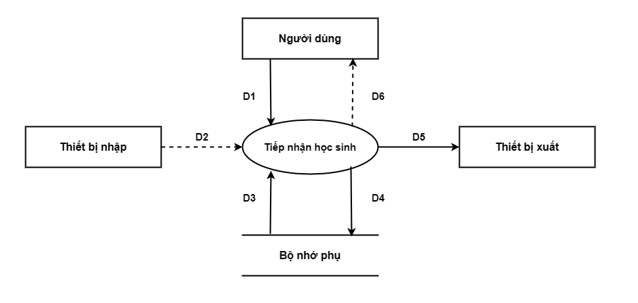
\includegraphics[width=1\textwidth]{dfd1} % Adjust width as needed
    \caption{Sơ đồ luồng dữ liệu cho yêu cầu Tiếp nhận học sinh}
\end{figure}


\item Mô tả các luồng dữ liệu
\begin{itemize}
\item D1: Thông tin học sinh (Họ và tên, Giới tính, Ngày sinh, Địa chỉ, Email, SĐT)
\item D2: Không có
\item D3: Tuổi tối thiểu, tối đa
\item D4: D1 
\item D5: D4
\item D6: Không có
\end{itemize}

\item Thuật toán
\begin{itemize}
\item B1: Nhận D1 từ người dùng
\item B2: Kết nối cơ sở dữ liệu
\item B3: Đọc D3 từ bộ nhớ phụ
\item B4: Tính tuổi học sinh
\item B5: Kiểm tra tuổi tối thiểu <= tuổi học sinh <= tuổi tối đa?
\item B6: Nếu không thỏa một trong các điều kiện trên thì => B9
\item B7: Lưu D4 xuống bộ nhớ phụ
\item B8: Xuất D5 ra máy in
\item B9: Đóng kết nối cơ sở dữ liệu
\item B10: Kết thúc
\end{itemize}

\end{enumerate}		
		
	\subsubsection{Lập danh sách lớp}
\begin{enumerate}[label=\alph*.]
\item Biểu mẫu và quy định

\begin{table}[H]
	\centering
	 \renewcommand{\arraystretch}{1.5}
	   \setlength{\tabcolsep}{20pt}
	 \begin{tabular}{|c|c|c|c|c|}
	 \hline
	 \multicolumn{5}{|c|}{\textbf{BM2: Danh sách lớp}} \\
	 \hline
	 Năm học:  & Khối:  & Lớp:  & \multicolumn{2}{|c|}{Sĩ số: \dotfill}\\
	 \hline
	 \textbf{STT} & \textbf{Họ tên} & \textbf{Giới tính} & \textbf{Năm sinh} & \textbf{Địa chỉ}\\
	 \hline
	 1 & & & &\\
	 \hline
	 2 & & & & \\
	 \hline
	 \end{tabular}
	\end{table}
\textbf{QĐ2: Có 3 khối lớp (10, 11, 12). Khối 10 có 4 lớp (10A1, 10A2, 10A3, 10A4). Khối 11 có 3 lớp (11A1, 11A2, 11A3). Khối 12 có 2 lớp (12A1, 12A2). Mỗi lớp không quá 40 học sinh.}	
\item Sơ đồ luồng dữ liệu
\begin{figure}[H] 
    \centering
    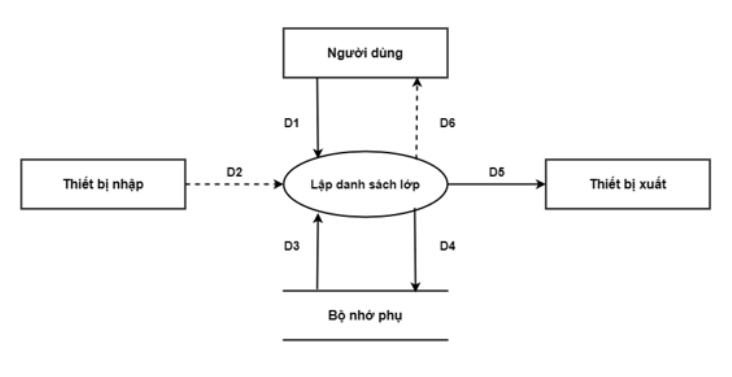
\includegraphics[width=1\textwidth]{dfd2} % Adjust width as needed
    \caption{Sơ đồ luồng dữ liệu cho yêu cầu Lập danh sách lớp }
    \label{fig:example} % Label for referencing the figure
\end{figure}	

\item Mô tả các luồng dữ liệu
\begin{itemize}
\item D1: Năm học, khối, lớp, sĩ số, họ tên, giới tính, năm sinh, địa chỉ
\item D2: Không có
\item D3: Danh sách năm học, khối, lớp, sĩ số tối đa của lớp
\item D4: D1
\item D5: D4
\item D6: Không có

\end{itemize}


\item Thuật toán
\begin{itemize}
\item B1: Nhận D1 từ người dùng
\item B2: Kết nối cơ sở dữ liệu
\item B3: Đọc D3 từ bộ nhớ phụ
\item B4: Kiểm tra năm có thuộc danh sách các năm hay không
\item B5: Kiểm tra khối có thuộc danh sách các khối hay không
\item B6: Kiểm tra lớp có thuộc danh sách các lớp hay không
\item B7: Tính số lượng học sinh thêm vào lớp
\item B8: Kiểm tra số lượng học sinh có vượt quá sĩ số tối đa hay không
\item B9: Nếu không thỏa mãn 1 trong các điều kiện trên thì đến B12
\item B10: Lưu D4 xuống bộ nhớ phụ
\item B11: Xuất D5 ra máy in
\item B12: Đóng kết nối cơ sở dữ liệu
\item B13: Kết thúc

\end{itemize}


\end{enumerate}	
	
	
	\subsubsection{Tra cứu học sinh}
	\begin{enumerate}[label=\alph*.]
\item Biểu mẫu và quy định

\begin{table}[H]
    \centering
    \renewcommand{\arraystretch}{1.5}
    \setlength{\tabcolsep}{12pt} % Adjust column spacing if needed
    \begin{tabular}{|c|c|c|c|c|c|}
    \hline
    \multicolumn{5}{|c|}{\textbf{BM3: Danh Sách Học Sinh}} \\  
    \hline
    
   \multicolumn{5}{|c|}{Năm học: \dotfill} \\  
   \hline
    
    \textbf{STT} & \textbf{Họ Tên} & \textbf{Lớp} & \textbf{TB Học Kỳ I} & \textbf{TB Học Kỳ II} \\  
    \hline
    1 & & & & \\  
    \hline
    2 & & & & \\  
    \hline
    \end{tabular}
\end{table}


\item Sơ đồ luồng dữ liệu
\begin{figure}[H] 
    \centering
    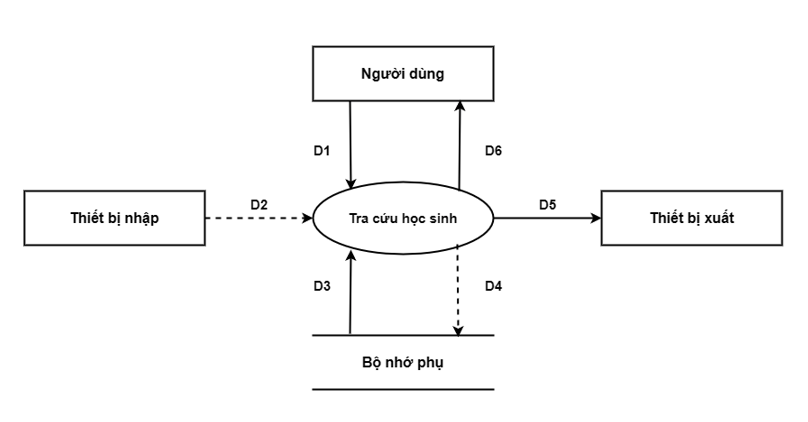
\includegraphics[width=1\textwidth]{dfd3} % Adjust width as needed
    \caption{Sơ đồ luồng dữ liệu cho yêu cầu Tra cứu học sinh }
    \label{fig:example} % Label for referencing the figure
\end{figure}	
\item Mô tả các luồng dữ liệu
\begin{itemize}
\item D1: Tiêu chuẩn tra cứu (Năm học, họ tên, lớp, trung bình HK1, trung bình HK2)
\item D2: Không có
\item D3: Danh sách học sinh thỏa tiêu chuẩn tra cứu
\item D4: Không có
\item D5: D3
\item D6: D5
\end{itemize}


\item Thuật toán
\begin{itemize}
\item B1: Nhận D1 từ người dùng
\item B2: Kết nối cơ sở dữ liệu
\item B3: Đọc D3 từ bộ nhớ phụ
\item B4: Xuất D5 ra máy in
\item B5: Trả D6 cho người dùng
\item B6: Đóng kết nối cơ sở dữ liệu
\item B7: Kết thúc
\end{itemize}


\end{enumerate}	
	
	\subsubsection{Nhận bảng điểm môn}	
	\begin{enumerate}[label=\alph*.]
\item Biểu mẫu và quy định

\begin{table}[H]
    \centering
    \renewcommand{\arraystretch}{1.5}
    \setlength{\tabcolsep}{12pt} % Adjust column spacing if needed
    \begin{tabular}{|c|c|c|c|c|}
    \hline
    \multicolumn{5}{|c|}{\textbf{BM4: Bảng Điểm Môn Học}} \\  
    \hline
    Năm học: & Khối: & Lớp: & Học kỳ:  & Môn:  \\  
    \hline
   \
    \textbf{STT} & \textbf{Họ Tên} & \textbf{Điểm 15'} & \textbf{Điểm 1 tiết} & \textbf{Điểm TB} \\  
    \hline
    1 & & & & \\  
    \hline
    2 & & & & \\  
    \hline
    \end{tabular}
\end{table}

\textbf{QĐ4: Có 2 học kỳ (I, II). Có 9 môn học (Toán, Lý, Hóa, Sinh, Sử, Địa, Văn, Đạo Đức, Thể Dục). 0 <= Điểm <= 10}

\item Sơ đồ luồng dữ liệu
\begin{figure}[H] 
    \centering
    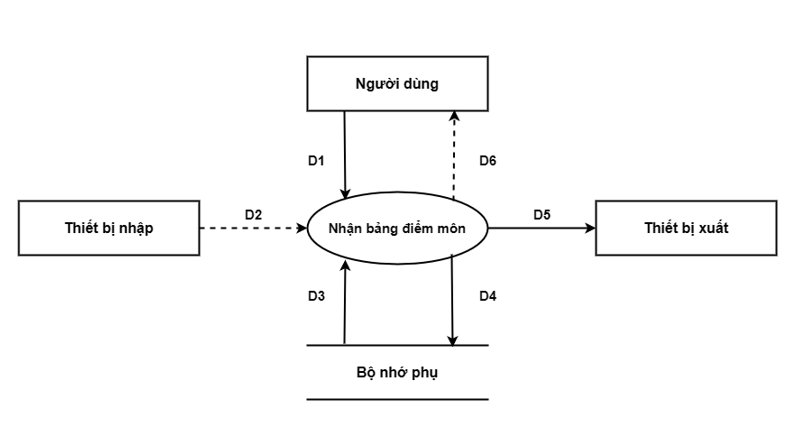
\includegraphics[width=1\textwidth]{dfd4} % Adjust width as needed
    \caption{Sơ đồ luồng dữ liệu cho yêu cầu Nhận bảng điểm môn }
    \label{fig:example} % Label for referencing the figure
\end{figure}	
\item Mô tả các luồng dữ liệu
\begin{itemize}
\item D1: Năm học, khối, lớp, học kỳ, môn, họ tên, các loại điểm
\item D2: Không có
\item D3: Danh sách năm học, khối, lớp, học kỳ, môn, các loại điểm, điểm tối thiểu, tối đa
\item D4: D1
\item D5: D4
\item D6: Không có
\end{itemize}


\item Thuật toán
\begin{itemize}
\item B1: Nhận D1 từ người dùng
\item B2: Kết nối cơ sở dữ liệu
\item B3: Đọc D3 từ bộ nhớ phụ
\item B4: Kiểm tra năm có thuộc danh sách các năm hay không
\item B5: Kiểm tra khối có thuộc danh sách các khối hay không
\item B6: Kiểm tra lớp có thuộc danh sách các lớp hay không
\item B7: Kiểm tra xem điểm tối thiểu <= điểm nhập <= điểm tối đa không
\item B8: Nếu không thỏa 1 trong các điều kiện thì B1
\item B9: Lưu D4 xuống bộ nhớ phụ
\item B10: Xuất D5 ra máy in
\item B11: Đóng kết nối cơ sở dữ liệu
\item B12: Kết thúc
\end{itemize}
\end{enumerate}	
	



	\subsubsection{Lập báo cáo tổng kết}
		\begin{enumerate}[label=\alph*.]
\item Biểu mẫu và quy định
\begin{table}[H]
    \centering
    \renewcommand{\arraystretch}{1.5}
    \setlength{\tabcolsep}{15pt} % Adjust column spacing if needed
    \begin{tabular}{|c|c|c|c|c|}
    \hline
    \multicolumn{5}{|c|}{\textbf{BM5.1: Báo Cáo Tổng Kết Môn}} \\  
    \hline
    Năm học: & \multicolumn{2}{|c|}{Môn:} & \multicolumn{2}{c|}{Học kỳ: } \\  
    \hline
    \textbf{STT} & \textbf{Lớp} & \textbf{Sĩ Số} & \textbf{Số Lượng Đạt} & \textbf{Tỉ Lệ} \\  
    \hline
    1 & & & & \\  
    \hline
    2 & & & & \\  
    \hline
    \end{tabular}
\end{table}
	

\begin{table}[H]
    \centering
    \renewcommand{\arraystretch}{1.5}
    \setlength{\tabcolsep}{15pt} % Adjust column spacing if needed
    \begin{tabular}{|c|c|c|c|c|}
    \hline
    \multicolumn{5}{|c|}{\textbf{BM5.2: Báo Cáo Tổng Kết Học Kỳ}} \\  
    \hline
      \multicolumn{2}{|c|}{Năm học: } &  \multicolumn{3}{|c|}{Học kỳ: } \\  
    \hline
    \textbf{STT} & \textbf{Lớp} & \textbf{Sĩ Số} & \textbf{Số Lượng Đạt} & \textbf{Tỉ Lệ} \\  
    \hline
    1 & & & & \\  
    \hline
    2 & & & & \\  
    \hline
    \end{tabular}
\end{table}

\textbf{QĐ5: Học sinh đạt môn/đạt nếu có điểm trung bình >= 5. } 	
\item Sơ đồ luồng dữ liệu
\begin{figure}[H] 
    \centering
    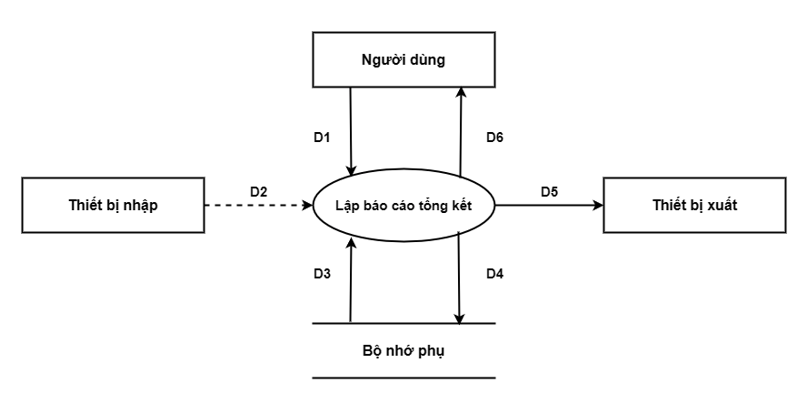
\includegraphics[width=1\textwidth]{dfd5} % Adjust width as needed
    \caption{Sơ đồ luồng dữ liệu cho yêu cầu Lập báo cáo tổng kết }
    \label{fig:example} % Label for referencing the figure
\end{figure}	
\item Mô tả các luồng dữ liệu
\begin{itemize}
\item D1: Năm học + Học kỳ
\item D2: Không có
\item D3: Danh sách xếp lớp và điểm của học sinh, điểm đạt môn/học kỳ
\item D4: D1 + Thông tin thống kê theo từng lớp trong học kỳ được chọn (Lớp, sĩ số, số lượng đạt, tỉ lệ)
\item D5: D4
\item D6: D5

\end{itemize}
\item Thuật toán
\begin{itemize}
\item B1: Nhận D1 từ người dùng
\item B2: Kết nối cơ sở dữ liệu
\item B3: Đọc D3 từ bộ nhớ phụ
\item B4: Tính điểm trung bình của học sinh trong từng lớp
\item B5: Đếm số lượng học sinh đạt (dựa vào điểm đạt môn/học kỳ) của từng lớp
\item B6: Tính tỉ lệ đạt dựa trên sĩ số và số học sinh đạt
\item B7: Lưu D4 xuống bộ nhớ phụ
\item B8: Xuất D5 ra máy in
\item B9: Trả D6 cho người dùng
\item B10: Đóng kết nối cơ sở dữ liệu
\item B11: Kết thúc
\end{itemize}

\end{enumerate}	
			


			\subsubsection{Thay đổi quy định}
			\begin{enumerate}[label=\alph*.]
\item Biểu mẫu và quy định

QĐ6: Người dùng có thể thay đổi các qui định như sau: 
\begin{itemize}
 \item QĐ1: Thay đổi tuổi tối thiểu, tuổi tối đa.
      \item QĐ2: Thay đổi sĩ số tối đa của các lớp, thay đổi số lượng và tên các lớp trong trường.
      \item QĐ4: Thay đổi số lượng và tên các môn học.
      \item QĐ5: Thay đổi điểm đạt môn/đạt
\end{itemize}


\item Sơ đồ luồng dữ liệu
\item Mô tả các luồng dữ liệu
\item Thuật toán
\end{enumerate}	
		
		\subsubsection{Thiết lập năm học}	
\begin{enumerate}
\item Biểu mẫu và quy định

\begin{table}[H]
\centering
\renewcommand{\arraystretch}{1.5}
\setlength{\tabcolsep}{15pt}
\begin{tabular}{|c|c|c|c|}
\hline
\multicolumn{4}{|c|}{\textbf{BM7: Thiết lập năm học}} \\
\hline
\multicolumn{2}{|p{5cm}|}{Năm bắt đầu: \dotfill}  & \multicolumn{2}{|p{5cm}|}{Năm kết thúc: \dotfill}  \\
\hline
\multicolumn{2}{|p{5cm}|}{Tuổi tối thiểu: \dotfill}  & \multicolumn{2}{|p{5cm}|}{Tuổi tối đa: \dotfill}  \\
\hline
\multicolumn{4}{|l|}{Điểm đạt: \dotfill} \\
\hline
\multicolumn{4}{|c|}{Các loại điểm} \\
\hline
STT & Tên loại điểm & Hệ số & \\
\hline 
1 & & & \\
\hline
2 & & & \\
\hline
\multicolumn{4}{|c|}{Các loại học lực} \\
\hline
STT & Tên học lực & Điểm tối thiểu & Điểm tối đa \\ 
\hline
1 & & & \\
\hline
2 & & & \\
\hline

\end{tabular}
\end{table}

QĐ7: Năm bắt đầu phải nhỏ hơn năm kết thúc. 1 <= Điểm đạt <= 10


\item Sơ đồ luồng dữ liệu
\begin{figure}[H] 
    \centering
    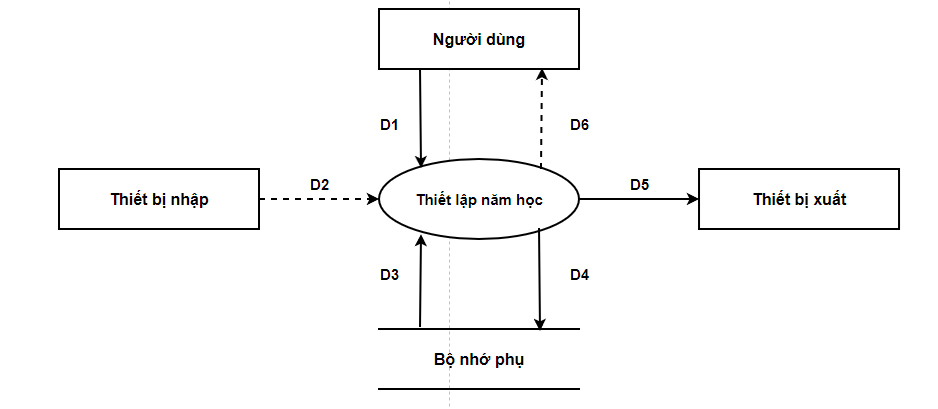
\includegraphics[width=1\textwidth]{dfd7} % Adjust width as needed
    \caption{Sơ đồ luồng dữ liệu cho yêu cầu Thiết lập năm học}
\end{figure}

\item Mô tả các luồng dữ liệu
\begin{itemize}
\item D1: Năm bắt đầu, năm kết thúc, tuổi tối thiểu, tuổi tối đa của học sinh, điểm đạt (điểm lên lớp), các loại điểm và hệ số, các loại học lực và khoảng điểm
\item D2: Không có
\item D3: Danh sách năm học, quy định về mức điểm.
\item D4: D1
\item D5: D4
\item D6: Không có
\end{itemize}
\item Thuật toán
\begin{itemize}
\item B1: Nhận D1 từ người dùng
\item B2: Kết nối cơ sở dữ liệu
\item B3: Đọc D3 từ bộ nhớ phụ
\item B4: Kiểm tra năm bắt đầu có nhỏ hơn năm kết thúc không
\item B5: Kiểm tra tuổi tối thiểu có nhỏ hơn tuổi tối đa không
\item B6: Kiểm tra điểm đạt có nằm trong khoảng quy đinh không
\item B7: Nếu không thoải một trong các điều kiện thì => B10
\item B8: Lưu D4 xuống bộ nhớ phụ
\item B9: Xuất D5 ra máy in
\item B10: Đóng kết nối cơ sở dữ liệu
\item B11: Kết thúc
\end{itemize}
\end{enumerate}		
		
		
		
			\subsubsection{Tạo khối}	
			\begin{enumerate}
\item Biểu mẫu và quy định
\begin{table}[H]
\centering
\renewcommand{\arraystretch}{1.5}
\setlength{\tabcolsep}{15pt}
\begin{tabular}{|p{5cm}|p{5cm}|}
\hline
\multicolumn{2}{|c|}{\textbf{BM8: Tạo khối}} \\
\hline
Tên khối: \dotfill & Thứ tự khối: \dotfill \\
\hline
\end{tabular}
\end{table}
\item Sơ đồ luồng dữ liệu

\begin{figure}[H] 
    \centering
    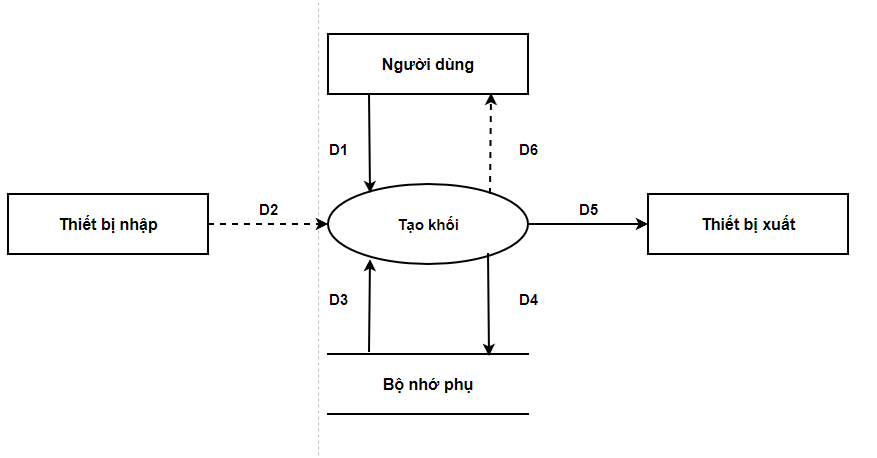
\includegraphics[width=1\textwidth]{dfd8} % Adjust width as needed
    \caption{Sơ đồ luồng dữ liệu cho yêu cầu Tạo khối}
\end{figure}

\item Mô tả các luồng dữ liệu
\begin{itemize}
\item D1: Tên khối, thứ tự khối
\item D2: Không có
\item D3: Danh sách khối
\item D4: D1
\item D5: D4
\item D6: Không có
\end{itemize}
\item Thuật toán
\begin{itemize}
\item B1: Nhận D1 từ người dùng
\item B2: Kết nối cơ sở dữ liệu
\item B3: Đọc D3 từ bộ nhớ phụ
\item B4: Kiểm tra thứ tự khối có trùng trong cơ sở dữ liệu không
\item B5: Nếu không thoải điều kiện thì => B8
\item B6: Lưu D4 xuống bộ nhớ phụ
\item B7: Xuất D5 ra máy in
\item B8: Đóng kết nối cơ sở dữ liệu
\item B9: Kết thúc
\end{itemize}
\end{enumerate}	
				\subsubsection{Tạo bộ môn}	
				\begin{enumerate}
\item Biểu mẫu và quy định

\begin{table}[H]
\centering
\renewcommand{\arraystretch}{1.5}
\setlength{\tabcolsep}{15pt}
\begin{tabular}{|p{10cm}|}
\hline
\multicolumn{1}{|c|}{\textbf{BM9: Tạo bộ môn}} \\  % Căn giữa tiêu đề
\hline
Tên bộ môn: \dotfill \\  
\hline
\end{tabular}
\end{table}


\item Sơ đồ luồng dữ liệu
\begin{figure}[H] 
    \centering
    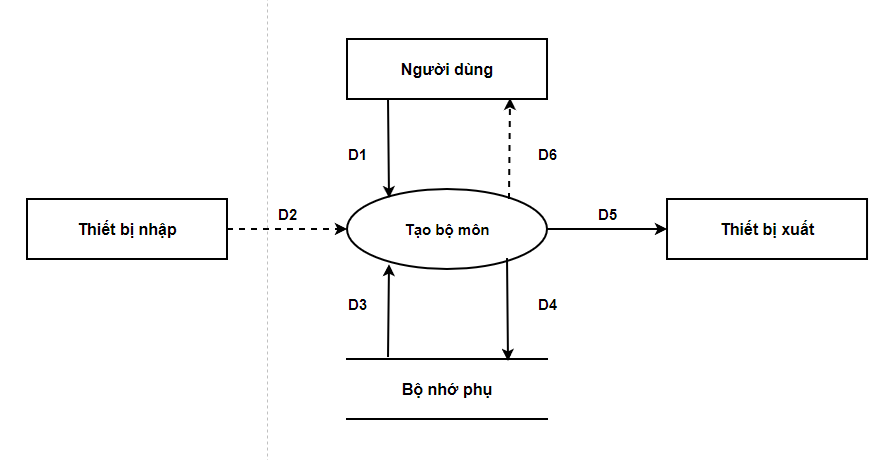
\includegraphics[width=1\textwidth]{dfd9} % Adjust width as needed
    \caption{Sơ đồ luồng dữ liệu cho yêu cầu Tạo bộ môn}
\end{figure}
\item Mô tả các luồng dữ liệu
\begin{itemize}
\item D1: Tên bộ môn
\item D2: Không có
\item D3: Danh sách bộ môn
\item D4: D1
\item D5: D4
\item D6: Không có
\end{itemize}
\item Thuật toán
\begin{itemize}
\item B1: Nhận D1 từ người dùng
\item B2: Kết nối cơ sở dữ liệu
\item B3: Đọc D3 từ bộ nhớ phụ
\item B4: Lưu D4 xuống bộ nhớ phụ
\item B5: Xuất D5 ra máy in
\item B6: Đóng kết nối cơ sở dữ liệu
\item B7: Kết thúc
\end{itemize}
\end{enumerate}	
					\subsubsection{Tạo lớp học}	
					\begin{enumerate}
\item Biểu mẫu và quy định

\begin{table}[H]
\centering
\renewcommand{\arraystretch}{1.5}
\setlength{\tabcolsep}{15pt}
\begin{tabular}{|p{5cm}|p{5cm}|}
\hline
\multicolumn{2}{|c|}{\textbf{BM10: Tạo lớp học}} \\  
\hline
Tên lớp: \dotfill  & Sĩ số: \dotfill \\
\hline
Năm học: \dotfill & Khối: \dotfill \\
\hline
\end{tabular}
\end{table}

QĐ10: Sĩ số > 0

\item Sơ đồ luồng dữ liệu
\begin{figure}[H] 
    \centering
    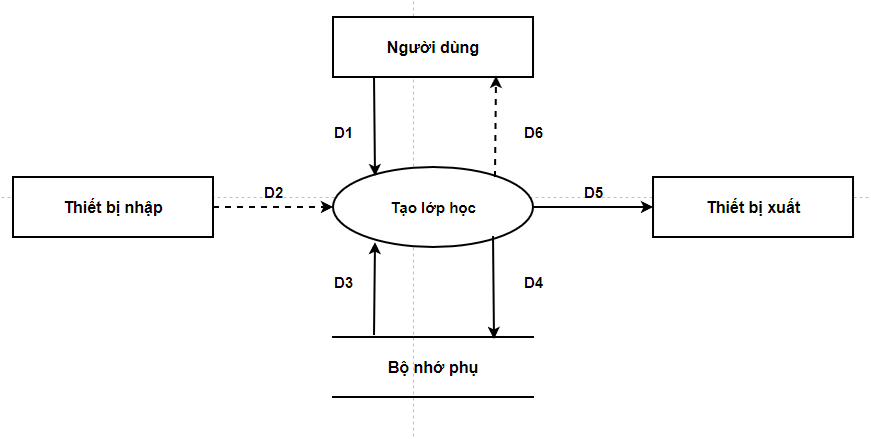
\includegraphics[width=1\textwidth]{dfd10} % Adjust width as needed
    \caption{Sơ đồ luồng dữ liệu cho yêu cầu Tạo lớp học}
\end{figure}

\item Mô tả các luồng dữ liệu
\begin{itemize}
\item D1: Tên lớp, khối, năm học, sĩ số
\item D2: Không có
\item D3: Danh sách khối, năm học, quy định về sĩ số
\item D4: D1
\item D5: D4
\item D6: Không có
\end{itemize}
\item Thuật toán
\begin{itemize}
\item B1: Nhận D1 từ người dùng
\item B2: Kết nối cơ sở dữ liệu
\item B3: Đọc D3 từ bộ nhớ phụ
\item B4: Kiểm tra năm có thuộc danh sách các năm không
\item B5: Kiểm tra khối có thuộc danh sách các khối không
\item B6: Kiểm tra sĩ số có nằm trong khoảng quy định không
\item B7: Nếu không thỏa một trong các điều kiện => B10
\item B8: Lưu D4 xuống bộ nhớ phụ
\item B9: Xuất D5 ra máy in
\item B10: Đóng kết nối cơ sở dữ liệu
\item B11: Kết thúc
\end{itemize}
\end{enumerate}	
						\subsubsection{Tạo môn học}	
						\begin{enumerate}
\item Biểu mẫu và quy định

\begin{table}[H]
\centering
\renewcommand{\arraystretch}{1.5}
\setlength{\tabcolsep}{15pt}
\begin{tabular}{|p{5cm}|p{5cm}|}
\hline
\multicolumn{2}{|c|}{\textbf{BM11: Tạo môn học}} \\  
\hline
Tên môn: \dotfill  & Điểm qua môn: \dotfill \\
\hline
Năm học: \dotfill & Khối: \dotfill \\
\hline
Bộ môn: \dotfill & \\
\hline
\multicolumn{2}{|c|}{Số lượng các loại điểm của môn} \\
\hline
Loại điểm & Số lượng \\
\hline
Thường xuyên & 3 \\
\hline
Giữa kỳ & 1 \\
\hline
... & ... \\
\hline
\end{tabular}
\end{table}

QĐ10: 0 <= Điểm qua môn <= 10

\item Sơ đồ luồng dữ liệu
\begin{figure}[H] 
    \centering
    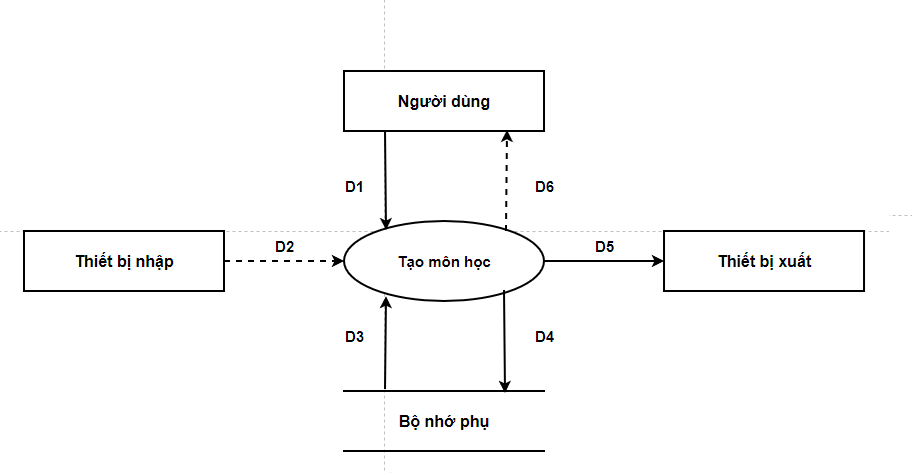
\includegraphics[width=1\textwidth]{dfd11} % Adjust width as needed
    \caption{Sơ đồ luồng dữ liệu cho yêu cầu Tạo môn học}
\end{figure}
\item Mô tả các luồng dữ liệu
\begin{itemize}
\item D1: Tên môn học, điểm qua môn, năm học, khối, bộ môn, số lượng các loại điểm của môn
\item D2: Không có
\item D3: Danh sách bộ môn, khối, năm học, danh sách các loại điểm của năm, quy định về điểm qua môn
\item D4: D1
\item D5: D4
\item D6: Không có
\end{itemize}
\item Thuật toán
\begin{itemize}
\item B1: Nhận D1 từ người dùng
\item B2: Kết nối cơ sở dữ liệu
\item B3: Đọc D3 từ bộ nhớ phụ
\item B4: Kiểm tra năm có thuộc danh sách các năm không
\item B5: Kiểm tra khối có thuộc danh sách các khối không
\item B6: Kiểm tra bộ môn có thuộc danh sách các bộ môn không
\item B7: Kiểm tra điểm qua môn có nằm trong khoảng quy định không
\item B8: Kiểm tra các loại điểm có giống với các danh sách các loại điểm của năm không
\item B9: Nếu không thoải một trong các điều kiện => B12
\item B10: Lưu D4 xuống bộ nhớ phụ
\item B11: Xuất D5 ra máy in
\item B12: Đóng kết nối cơ sở dữ liệu
\item B13: Kết thúc
\end{itemize}
\end{enumerate}	
							\subsubsection{Cấp tài khoản giáo viên}	
							\begin{enumerate}
\item Biểu mẫu và quy định

\begin{table}[H]
\centering
\renewcommand{\arraystretch}{1.5}
\setlength{\tabcolsep}{15pt}
\begin{tabular}{|p{5cm}|p{5cm}|}
\hline
\multicolumn{2}{|c|}{\textbf{BM12: Cấp tài khoản giáo viên}} \\  
\hline
Họ và tên: \dotfill  & Tên tài khoản: \dotfill \\
\hline
Email: \dotfill & Mật khẩu: \dotfill \\
\hline
Bộ môn: \dotfill & \\
\hline
\end{tabular}
\end{table}


\item Sơ đồ luồng dữ liệu
\begin{figure}[H] 
    \centering
    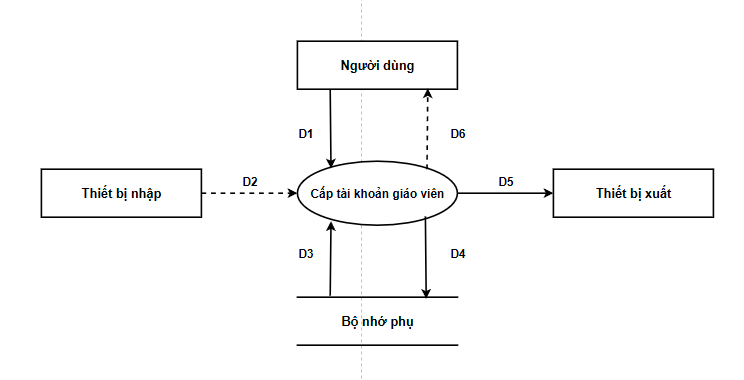
\includegraphics[width=1\textwidth]{dfd12} % Adjust width as needed
    \caption{Sơ đồ luồng dữ liệu cho yêu cầu Cấp tài khoản giáo viên}
\end{figure}
\item Mô tả các luồng dữ liệu
\begin{itemize}
\item D1: Họ và tên, tên tài khoản, email, mật khẩu, bộ môn
\item D2: Không có
\item D3: Danh sách các tài khoản, bộ môn
\item D4: D1
\item D5: D4
\item D6: Không có
\end{itemize}
\item Thuật toán
\begin{itemize}
\item B1: Nhận D1 từ người dùng
\item B2: Kết nối cơ sở dữ liệu
\item B3: Đọc D3 từ bộ nhớ phụ
\item B4: Kiểm tra xem tên tài khoản có bị trùng không
\item B5: Kiểm tra bộ môn có nằm trong danh sách bộ môn không
\item B6: Nếu không thỏa 1 trong các điều kiện => B9
\item B7: Lưu D4 xuống bộ nhớ phụ
\item B8: Xuất D5 ra máy in
\item B9: Đóng kết nối cơ sở dữ liệu
\item B10: Kết thúc
\end{itemize}
\end{enumerate}	
								\subsubsection{Phân công giảng dạy}	
								\begin{enumerate}
\item Biểu mẫu và quy định

\begin{table}[H]
	\centering
	 \renewcommand{\arraystretch}{1.5}
	   \setlength{\tabcolsep}{15pt}
	 \begin{tabular}{|c|c|c|c|c|c|}
	 \hline
	 \multicolumn{6}{|c|}{\textbf{BM13: Phân công giảng dạy}} \\
	 \hline
	 \multicolumn{2}{|c|}{Năm học: } & \multicolumn{2}{|c|}{Khối: } & \multicolumn{2}{|c|}{Bộ môn: } \\
	 \hline
	 \textbf{STT} & \textbf{Giáo viên} & \textbf{Lớp} & \textbf{Môn} & \textbf{Thứ} & \textbf{Tiết} \\
	 \hline
	 1 & & & & & \\
	 \hline
	 2 & & & & &\\
	 \hline
	 \end{tabular}
	\end{table}

QĐ13: Giáo viên dạy môn nào thì phải cùng thuộc bộ môn với môn đó

\item Sơ đồ luồng dữ liệu
\begin{figure}[H] 
    \centering
    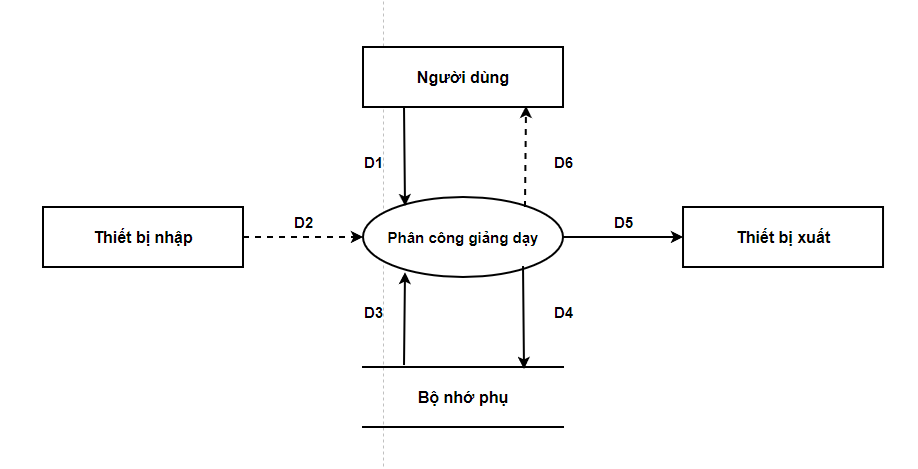
\includegraphics[width=1\textwidth]{dfd13} % Adjust width as needed
    \caption{Sơ đồ luồng dữ liệu cho yêu cầu Phân công giảng dạy}
\end{figure}
\item Mô tả các luồng dữ liệu
\begin{itemize}
\item D1: Năm học, khối, bộ môn, họ tên giáo viên, lớp, môn, thứ, tiết
\item D2: Không có
\item D3: Danh sách năm học, khối, bộ môn, lớp, môn, giáo viên
\item D4: D1
\item D5: D4
\item D6: Không có 
\end{itemize}
\item Thuật toán
\begin{itemize}
\item B1: Nhận D1 từ người dùng
\item B2: Kết nối cơ sở dữ liệu
\item B3: Đọc D3 từ bộ nhớ phụ
\item B4: Kiểm tra năm có thuộc danh sách các năm không
\item B5: Kiểm tra khối có thuộc danh sách các khối không
\item B6: Kiểm tra bộ môn có thuộc danh sách các bộ môn không
\item B7: Kiểm tra lớp có thuộc danh sách các lớp không
\item B8: Kiểm tra môn có thuộc danh sách các môn không
\item B9: Nếu không thỏa một trong các điều kiện => B12
\item B10: Lưu D4 xuống bộ nhớ phụ
\item B11: Xuất D5 ra máy in
\item B12: Đóng kết nối cơ sở dữ liệu
\item B13: Kết thúc
\end{itemize}
\end{enumerate}	
								
							
		

\section{THIẾT KẾ HỆ THỐNG}
	\subsection{Kiến trúc hệ thống}
	\subsection{Mô tả các thành phần trong hệ thống}

\section{THIẾT KẾ DỮ LIỆU}
	\subsection{Thuật toán thiết kế dữ liệu}
	\subsection{Sơ đồ logic hoàn chỉnh}
	\subsection{Danh sách các bảng dữ liệu trong sơ đồ}
	\subsection{Mô tả từng bảng dữ liệu}

\section{THIẾT KẾ GIAO DIỆN}
	\subsection{Sơ đồ liên kết các màn hình}
	\subsection{Danh sách các màn hình}
	\subsection{Mô tả các màn hình}

\section{CÀI ĐẶT VÀ THỬ NGHIỆM}

\section{KẾT LUẬN}
	\subsection{Ưu điểm}


	\subsection{Khuyết điểm}
	\subsection{Hướng phát triển}

\section{TÀI LIỆU THAM KHẢO}

\section{BẢNG PHÂN CÔNG CÔNG VIỆC}

\end{document}
